\exercisesection{Exercises for § 4}

In the exercises below, (W, S) denotes a Coxeter system. We assume that S is finite; its cardinal is called the rank of (W, S). We identify W with a subgroup of \(\mathbf{GL}(\mathbf{E})\) by means of \(\sigma\) (cf.~nos. 3 and 4).

\begin{enumerate}
\def\labelenumi{\arabic{enumi})}
\item
  Let \(E^{0}\) be the orthogonal complement of E with respect to the form \(B_{M}\) . Show that \(E^{0}\) is the radical of the W-module E (Algebra, Chap. VIII, §6, no. 2), and that \(E/E^{0}\) is the direct sum of m absolutely simple, pairwise non-isomorphic modules, where m is the number of connected components of the graph of S.
\item
  \begin{enumerate}
  \def\labelenumii{\alph{enumii})}
  \tightlist
  \item
    Let \(\Gamma_w\) be the set of extremal generators of the cone \(w(\mathbf{C})\) and let A be the union of the \(\Gamma_w\) for \(w \in \mathbf{W}\) . Show that A, equipped with the set \(\{\Gamma_w | w \in \mathbf{W}\}\) , is a building (Chap. IV, §1, Exerc. 15). Show that the map \(j\) from the apartment \(\mathrm{A}_0\) associated to the Coxeter system (W,S) (Chap. IV, §1, Exerc. 16) to A that transforms the point \(w\mathrm{W}^{(s)}\) of \(\mathrm{A}_0\) (for \(w \in \mathbf{W}\) and \(s \in \mathbf{S}\) ) to the generator \(w(\mathbf{R}e_s)\) , is an isomorphism from \(\mathrm{A}_0\) to A, compatible with the action of W. Show that, if \(t = wsw^{-1}\) , with \(w \in \mathbf{W}\) and \(s \in \mathbf{S}\) , the image under \(j\) of the wall \(\mathbf{L}_t\) defined by \(t\) (resp. of a half of \(\mathrm{A}_0\) defined by \(\mathbf{L}_t\) ) (loc. cit.) is the set of elements of A contained in the hyperplane (resp. the closed half-space) that is the transform by \(\sigma^*(w)\) of the hyperplane \(e_s = 0\) (resp. of one of the closed half-spaces \(e_s \geqslant 0\) or \(e_s \leqslant 0\) ).
  \end{enumerate}
\end{enumerate}

\begin{enumerate}
\def\labelenumi{\alph{enumi})}
\setcounter{enumi}{1}
\item
  Show that W is finite if and only if there exists an element \(w_{0} \in W\) such that \(w_{0}(C) = -C\) . This element \(w_{0}\) is then unique and is the longest element of W (use Exerc. 22 of Chap. IV, §1). Show that in that case \(j(-a) = -j(a)\) for all \(a \in A_{0}\) (cf.~Exerc. 22 c) of Chap. IV, §1).
\item
  Show that W is finite if and only if the cone U formed by taking the union of the cone closures \(w(\overline{C})\) for \(w \in W\) is equal to the whole of \(E^{*}\) (if W is finite, use b) and the convexity of U. If \(U = E^{*}\) , consider an element \(w \in W\) such that \(w(\overline{C}) \cap (-C) \neq \varnothing\) and show that \(w(C) = -C\) .
\item
  Let H be a finite subgroup of W. Show that there exists a subset X of S such that \(W_{X}\) is finite and contains a conjugate of H. (Argue by induction on \(\operatorname{Card}(S)\) . Let \(x \in C\) and \(\overline{x} = \sum_{h \in H} h(x)\) . Show, by using c) above, that W is finite if \(\overline{x} = 0\) . If \(\overline{x} \neq 0\) , there exist \(w \in W\) and \(Y \subset S\) , \(Y \neq S\) , such that \(w(\overline{x})\) belongs to \(C_{Y}\) (in the notation of no. 6), and hence \(H \subset w^{-1}W_{Y}w\) ; apply the induction hypothesis to Y.)
\end{enumerate}

\begin{enumerate}
\def\labelenumi{\arabic{enumi})}
\setcounter{enumi}{2}
\tightlist
\item
  Assume that \((\mathbf{W},\mathbf{S})\) is irreducible.
\end{enumerate}

\begin{enumerate}
\def\labelenumi{\alph{enumi})}
\item
  Show that the commutant of the W-module E reduces to the homotheties.
\item
  Show that the centre of W reduces to \(\{1\}\) if W is infinite or if W is finite and the longest element \(w_{0}\) (cf.~Exerc. 2) is \(\neq -1\) . If W is finite and \(w_{0} = -1\) , the centre of W is \(\{1, w_{0}\}\) .
\item
  Show that any element \(w \neq 1\) of W such that \(wSw^{-1} = S\) transforms C to -C (show that \(w(e_s) = -e_{wsw^{-1}}\) , first for some \(s \in S\) , and then for all \(s \in S\) ). Deduce (Exerc. 2) that such an element exists only if W is finite and that it is then equal to \(w_0\) .
\end{enumerate}

\begin{enumerate}
\def\labelenumi{\arabic{enumi})}
\setcounter{enumi}{3}
\tightlist
\item
  Assume that \(\operatorname{Card}(S) = 3\) . If \(s \in S\) , let \(a(s) = m(u, v)\) , where \(\{u, v\} = S - \{s\}\) . Let \(A = \sum_{s \in S} 1 / a(s)\) .
\end{enumerate}

\begin{enumerate}
\def\labelenumi{\alph{enumi})}
\item
  If A \textgreater{} 1, show that \(B_{M}\) is non-degenerate and positive (in which case W is finite).
\item
  If \(\mathrm{A} = 1\) , show that \(\mathsf{B}_{\mathsf{M}}\) is degenerate and positive.
\item
  If \(\mathbf{A} < 1\) , show that \(\mathbf{B}_{\mathbf{M}}\) is non-degenerate and of signature (2,1) (cf.~Algebra, Chap. IX, §7, no. 2).
\end{enumerate}

Show that, in case \(a\) ), the order \(q\) of \(W\) is given by the formula \(q = 4 / (A - 1)\) (use Exerc. 5 of §3).

\begin{enumerate}
\def\labelenumi{\arabic{enumi})}
\setcounter{enumi}{4}
\tightlist
\item
  Let A be the subring of R generated by the numbers 2. \(\cos(\pi/m(s, s'))\) . Show that A is a free Z-module of finite type, and that the matrices of the \(\sigma(w)\) for \(w \in W\) have their coefficients in A. Deduce that the coefficients of the characteristic polynomials of the \(\sigma(w)\) are algebraic integers.
\end{enumerate}

¶ 6) a) Let m be an integer ≥ 2, or +∞. Show that \(4 \cos^{2} \frac{\pi}{m} \in Z\) is equivalent to \(m \in \{2, 3, 4, 6, +\infty\}\) .

\begin{enumerate}
\def\labelenumi{\alph{enumi})}
\setcounter{enumi}{1}
\item
  Let \(\Gamma\) be a lattice in E, i.e.~a discrete subgroup of E of rank dim E. Show that, if \(\Gamma\) is stable under W, the integers \(m(s, s')\) for \(s \neq s'\) all belong to the set \(\{2, 3, 4, 6, +\infty\}\) . (Observe that \(\operatorname{Tr}(\sigma(w)) \in \mathbf{Z}\) for all \(w \in W\) ; apply this result to \(w = ss'\) , and use \(a\) ) above.)
\item
  Assume that \(m(s, t) \in \{2, 3, 4, 6, +\infty\}\) for \(s \neq t \in S\) . A family \((x_s)_{s \in S}\) of positive real numbers is called radical if it satisfies the following conditions:
\end{enumerate}

\[
m (s, t) = 3 \Longrightarrow x _ {s} = x _ {t}
\]

\[
m (s, t) = 4 \Longrightarrow x _ {s} = \sqrt {2}. x _ {t} \text { or } x _ {t} = \sqrt {2}. x _ {s}
\]

\[
m (s, t) = 6 \Longrightarrow x _ {s} = \sqrt {3}. x _ {t} \text {or} x _ {t} = \sqrt {3}. x _ {s}.
\]

\[
m (s, t) = + \infty \Longrightarrow x _ {s} = x _ {t} \quad \text { or } x _ {s} = 2 x _ {t} \text { or } x _ {t} = 2 x _ {s}.
\]

If \((x_{s})_{s\in S}\) is such a family, put \(\alpha_{s} = x_{s}e_{s}\) . Show that

\[
\sigma_ {s} (\alpha_ {t}) = \alpha_ {t} - n (s, t) \alpha_ {s}, \quad \text { with } n (s, t) \in \mathbf {Z}.
\]

Deduce that the lattice \(\Gamma\) with basis \((\alpha_s)_{s\in S}\) is stable under W.

  \(d)\) With the assumptions in \(c\) ), suppose that the graph of \((\mathrm{W},\mathrm{S})\) is a forest. Show that in that case there exists at least one radical family \((x_{s})\) . (Argue by induction on \(\operatorname{Card}(S)\) ; apply the induction hypothesis to \(S - \{s_{0}\}\) , where \(s_{0}\) is a terminal vertex of the graph of S.)

\begin{enumerate}
\def\labelenumi{\alph{enumi})}
\setcounter{enumi}{4}
\tightlist
\item
  With the assumptions in c), suppose that the graph of (W, S) is a circuit. Let \(n_{4}\) (resp. \(n_{6}\) ) be the number of arrows \(\{s, t\}\) of this graph whose coefficient \(m(s, t)\) is equal to 4 (resp. 6). Show that a radical family exists if and only if \(n_{4}\) and \(n_{6}\) are both even. If this condition is not satisfied, show that no lattice of E is stable under W (if \(S = \{s_{1}, \ldots, s_{n}\}\) , with \(s_{i}\) linked to \(s_{i+1}\) for \(1 \leqslant i \leqslant n - 1\) , and \(s_{n}\) linked to \(s_{1}\) , put \(c = s_{1} \ldots s_{n}\) and show that \(\operatorname{Tr}(\sigma(c))\) is not an integer).
\end{enumerate}

\begin{enumerate}
\def\labelenumi{\arabic{enumi})}
\setcounter{enumi}{6}
\tightlist
\item
  Assume that \((W, S)\) is irreducible and that \(B_{M}\) is positive.
\end{enumerate}

\begin{enumerate}
\def\labelenumi{\alph{enumi})}
\item
  Show that, for any subset \(\mathbf{T}\) of \(S\) distinct from \(S\) , the group \(W_{T}\) is finite (use Th. 2 as well as Lemma 4 of §3, no. 5).
\item
  Show that, if \(\operatorname{Card}(S) \geqslant 3\) , the \(m(s, s')\) are all finite.
\item
  Assume that W is infinite. Show that, if \(T \subset S\) , \(T \neq S\) , the group \(\sigma(W_{T})\) leaves stable a lattice in \(R^{T}\) . Deduce that, if \(\text{Card}(S) \geqslant 3\) , the \(m(s, s')\) , \(s \neq s'\) , all belong to the set \(\{2, 3, 4, 6\}\) (use Exerc. 6).
\end{enumerate}

\begin{enumerate}
\def\labelenumi{\arabic{enumi})}
\setcounter{enumi}{7}
\item
  Let \(s \in S\) and \(w \in W\) . Show that, if \(l(ws) > l(w)\) , the element \(w(e_s)\) is a linear combination with coefficients \(\geqslant 0\) of the \(e_t\) for \(t \in S\) ; show that, if \(l(ws) < l(w)\) , \(w(e_s)\) is a linear combination with coefficients \(\leqslant 0\) of the \(e_t\) . (Apply property \((\mathbf{P}_n)\) of no. 4 to \(w^{-1}\) , and argue by polarity.)
\item
  Show that the intersection of the subgroups of W of finite index reduces to the identity element (use Exerc. 5). Deduce that there exists a subgroup of W of finite index that contains no element of finite order other than the identity element. (Use Exerc. 2 d.)
\end{enumerate}

¶ 10) Let G be a closed subgroup of GL(E) containing W. Assume that G is unimodular (Integration, Chap. VII, §1, no. 3). Let D be a half-line of E* contained in C, and let GD be the stabiliser of D in G.

\begin{enumerate}
\def\labelenumi{\alph{enumi})}
\item
  Let \(\Delta\) be the set of elements \(g \in G\) such that \(g(D) \subset C\) . Show that \(\Delta\) is open, stable under right multiplication by \(G_D\) , and that the composite map \(\Delta \to G \to W \backslash G\) is injective, \(W \backslash G\) denoting the homogeneous space of right cosets of \(G\) with respect to \(W\) .
\item
  Let \(\mu\) be a Haar measure on G. Show that, if \(\mu(\Delta)\) is finite, the subgroup \(G_{D}\) is compact. (Let K be a compact neighbourhood of the identity element contained in \(\Delta\) ; show that there exist finitely many elements \(h_i \in G_D\) such that every set of the form \(Kh\) , with \(h \in G_D\) , meets one of the \(Kh_i\) ; deduce that \(G_D\) is contained in the union of the \(K^{-1}K.h_i\) , and hence is compact.)
\item
  Let \(\nu\) be a non-zero positive measure on \(W\backslash G\) invariant under \(G\) . Show that, if \(\nu(W\backslash G) < \infty\) , then \(G_{D}\) is compact.
\end{enumerate}

¶ 11) Let H be the subset of \(\mathbf{R}^n\) consisting of the points \(x = (x_0, \ldots, x_{n-1})\) for which the form

\[
\mathrm{B} (x) = - x _ {0} ^ {2} + x _ {1} ^ {2} + \dots + x _ {n - 1} ^ {2}
\]

is \textless{} 0, and let PH be the image of H in the projective space \(\mathbf{P}_{n-1}(\mathbf{R})\) . Let G be the orthogonal group of the form B.

\begin{enumerate}
\def\labelenumi{\alph{enumi})}
\item
  Show that PH is a homogeneous space of G, that the stabiliser of a point is compact, and that G acts properly on PH.
\item
  Let \(\omega\) and \(\Omega\) be the differential forms on H defined by the formulas
\end{enumerate}

\[
\begin{array}{c} \omega = \sum_ {i = 0} ^ {n - 1} (- 1) ^ {i} x _ {i} d x _ {0} \wedge \dots \wedge d x _ {i - 1} \wedge d x _ {i + 1} \wedge \dots \wedge d x _ {n - 1} \\ \Omega = \frac {\omega}{(- \mathrm{B} (x)) ^ {n / 2}}. \end{array}
\]

Show that \(\Omega\) is the inverse image under the canonical projection \(\pi:H\to PH\) of a differential form \(\tilde{\Omega}\) on PH. Show that the positive measure \(\nu\) associated to \(\tilde{\Omega}\) (Differentiable Varieties R, 2nd part) is invariant under G, and that it is the only such measure, up to a scalar factor.

\begin{enumerate}
\def\labelenumi{\alph{enumi})}
\setcounter{enumi}{2}
\tightlist
\item
  Let C be an open simplicial cone with vertex 0 in \(\mathbf{R}^n\) (§1, no. 6). Assume that C is contained in H, and denote by PC the image of C under \(\pi: \mathrm{H} \to \mathrm{PH}\) . Show that, if \(n \geqslant 3\) , then \(\nu(\mathrm{PC}) < \infty\) (identify PH with the subspace of \(\mathbf{R}^{n-1}\) consisting of the \((x_1, \ldots, x_{n-1})\) such that \(\sum_{i=1}^{n-1} x_i^2 < 1\) , and determine the measure corresponding to \(\nu\) on this subspace). Show that PC is relatively compact in PH if and only if \(\overline{\mathbf{C}}\) is contained in H.
\end{enumerate}

¶ 12) Assume that the form \(x.y = \mathrm{B}_{\mathrm{M}}(x,y)\) is non-degenerate and that W is infinite. Identify E with its dual \(\mathrm{E}^*\) by means of \(\mathrm{B}_{\mathrm{M}}\) ; in particular, denote by \((e_s^*)\) the basis of E dual to the basis \((e_s)\) , and by C the interior of the simplicial cone \(\overline{\mathbf{C}}\) generated by the \(e_s^*\) . Let G be the orthogonal group of \(\mathrm{B}_{\mathrm{M}}\) , and let \(\mu\) be a Haar measure on G; the group G is unimodular and contains W.

\begin{enumerate}
\def\labelenumi{\alph{enumi})}
\tightlist
\item
  Show that, if \(\nu (\mathrm{W}\backslash \mathrm{G}) < \infty\) (where \(\nu\) is a non-zero positive measure invariant under \(\mathbf{G}\) ), the form \(\mathrm{B_M}\) is of signature \((n - 1,1)\) , with
\end{enumerate}

\[
n = \dim (\mathrm{E}) = \operatorname{Card} (\mathrm{S}),
\]

and that \(x.x < 0\) for all \(x \in C\) .

(Let \(x \in C\) be such that \(x.x \neq 0\) , and let \(\mathrm{L}_x\) be the hyperplane orthogonal to \(x\) . Show, by using Exerc. 10, that the restriction of \(\mathrm{B}_{\mathrm{M}}\) to \(\mathrm{L}_x\) is either positive or negative; show that the second case implies that \(\mathrm{B}_{\mathrm{M}}\) is of signature \((1, n - 1)\) and that this is impossible. Deduce that \(x.x \leqslant 0\) for all \(x \in C\) , and hence \(x.x < 0\) since C is open.)

\begin{enumerate}
\def\labelenumi{\alph{enumi})}
\setcounter{enumi}{1}
\item
  Conversely, assume that \(B_{M}\) is of signature \((n-1,1)\) and x.x\textless0 for all \(x\in C\) (in which case W, or (W,S), or the corresponding Coxeter graph, is said to be of hyperbolic type). Let H be the set of \(x\in E\) such that x.x\textless0, and let \(H_{+}\) be the connected component of H containing C. Show that H is the disjoint union of \(H_{+}\) and \(H_{-}=-H_{+}\) , and that \(H_{-}\) is contained in the simplicial cone generated by \((e_{s})_{s\in S}\) (use the fact that \(H_{-}\) is the polar of \(H_{+}\) ). Show that \(H_{+}\) and \(H_{-}\) are stable under W.
\item
  Retain the notation and assumptions of b). Let f be the linear form on E defined by \(f(e_{s}) = 1\) for all \(s \in S\) . If \(x \in H\) , put \(\varphi(x) = f(x)^{2}/(x.x)\) . If PH denotes the image of the cone H in the projective space \(\mathbf{P}(\mathbf{E})\) , the function \(\varphi\) defines a function \(\tilde{\varphi}\) on PH. Show that the map
\end{enumerate}

\[
\left. \tilde {\varphi}: \mathrm{PH} \rightarrow ] - \infty , 0 ] \right.
\]

is proper. Deduce that, for all \(x \in H_{+}\) , the functions \(w \mapsto \varphi(w.x)\) and \(w \mapsto f(w.x)\) attain their maximum for a value \(w_{1} \in W\) (use the fact that G acts properly on PH, cf.~Exerc. 11, and that W is discrete in G); show that these properties are equivalent to \(w_{1}(x) \in \overline{\mathbf{C}}\) . Deduce that \(\overline{C} \cap H_{+}\) is a fundamental domain for the action of W in \(H_{+}\) , and that the image of this fundamental domain in PH has finite measure for the invariant measure \(\nu\) on PH (use Exerc. 11). Conclude that \(\nu(\mathrm{W} \backslash \mathrm{G}) < \infty\) . Show that \(W \backslash G\) is compact if and only if \(\overline{C}\) is contained in \(H_{+}\) , i.e.~if \(e_{s}^{*}.e_{s}^{*} < 0\) for all \(s \in S\) (in which case W, or (W,S), or the corresponding Coxeter graph, is said to be of compact hyperbolic type).

¶ 13) Show that (W, S) is of hyperbolic type (cf.~Exerc. 12) if and only if the following two conditions are satisfied:

\((H_{1})\) The form \(B_{M}\) is not positive.

\((H_{2})\) For any subset T of S distinct from S, the form \(B_{M(T)}\) associated to the Coxeter system \((W_{T}, T)\) is positive.

(If (W,S) is of hyperbolic type, we have seen that \(e_s^*.e_s^* \leqslant 0\) for all \(s \in S\) , the notation being that of Exerc. 12. The restriction of \(B_M\) to the hyperplane \(E(s)\) orthogonal to \(e_s^*\) is thus \(\geqslant 0\) ; since \(E(s)\) is generated by the \(e_t\) for \(t \neq s\) , \((H_2)\) follows. Conversely, assume that \((H_1)\) and \((H_2)\) are satisfied; let \(x = \sum_{s} a_s e_s\) be an element of E such that \(x.x < 0\) ; let \(x_+\) (resp. \(x_-\) ) be the sum of the \(a_s e_s\) for which \(a_s\) is \(> 0\) (resp. \(\leqslant 0\) ); show that either \(x_+.x_+ < 0\) or \(x_-.x_- < 0\) . If V denotes the open simplicial cone generated by the \(e_s\) , and H the set of \(x \in E\) such that \(x.x < 0\) , deduce that there exists a connected component \(H_0\) of H that meets V; by using \((H_2)\) , show that \(H_0\) does not meet the walls of V, so \(H_0 \subset V\) . Deduce that the form \(B_M(x,y) = x.y\) is non-degenerate of signature ( \(n-1,1\) ), and that C is contained in \(-H_0\) , hence the fact that (W,S) is of hyperbolic type.)

\begin{enumerate}
\def\labelenumi{\arabic{enumi})}
\setcounter{enumi}{13}
\tightlist
\item
  Show that \((\mathrm{W},\mathrm{S})\) is of compact hyperbolic type (Exerc. 12) if and only if the following two conditions are satisfied:
\end{enumerate}

\((H_{1})\) The form \(B_{M}\) is not positive.

(HC) For any subset T of S distinct from S, the group \(W_{T}\) is finite (i.e.~the form \(B_{\mathsf{M}(T)}\) is non-degenerate and positive).

(Use Exercs. 12 and 13.)

In particular, a Coxeter system of hyperbolic type of rank 3 is of compact hyperbolic type if and only if the \(m(s, s')\) are all finite (cf.~Exerc. 4).

¶ 15) *a) Show that the nine Coxeter graphs below \(^{7}\) are of compact hyperbolic type, and that they are, up to isomorphism, the only graphs of rank 4 with this property (use the classification of Chap. VI, § 4):

\pandocbounded{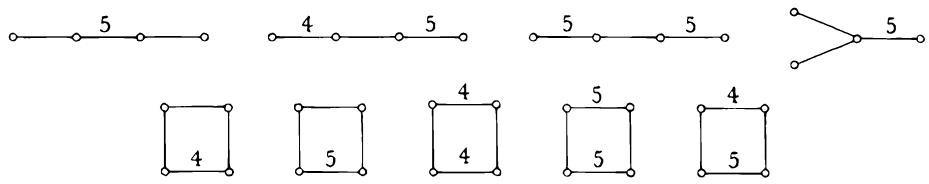
\includegraphics[keepaspectratio]{images/part001_8fab2eba.jpg}}

\begin{enumerate}
\def\labelenumi{\alph{enumi})}
\setcounter{enumi}{1}
\tightlist
\item
  The same question for rank 5, the list consisting of the following five graphs:
\end{enumerate}

\pandocbounded{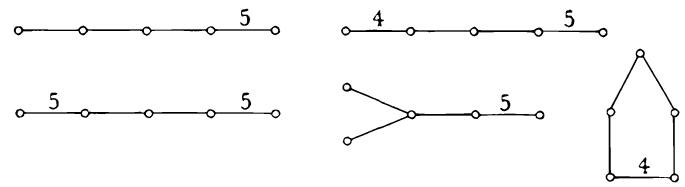
\includegraphics[keepaspectratio]{images/part001_6b3cac07.jpg}}

\begin{enumerate}
\def\labelenumi{\alph{enumi})}
\setcounter{enumi}{2}
\tightlist
\item
  Show that there is no graph of compact hyperbolic type of rank \(\geqslant 6\) .*
\end{enumerate}

\begin{enumerate}
\def\labelenumi{\arabic{enumi})}
\setcounter{enumi}{15}
\tightlist
\item
  *Show that any Coxeter graph of hyperbolic type of rank \(\geqslant 4\) that has an edge with coefficient 6 is isomorphic to one of the following eleven graphs (which are non-compact and of rank 4):
\end{enumerate}

\pandocbounded{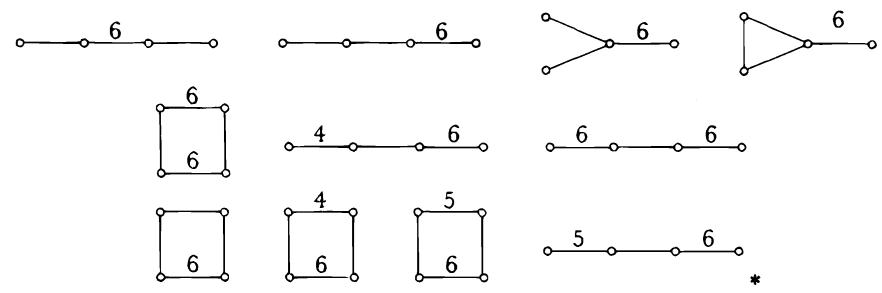
\includegraphics[keepaspectratio]{images/part001_2926a96c.jpg}}

\begin{enumerate}
\def\labelenumi{\arabic{enumi})}
\setcounter{enumi}{16}
\tightlist
\item
  *Show that the hyperbolic Coxeter graphs of higher rank are the following three graphs (which are of rank 10):
\end{enumerate}

\pandocbounded{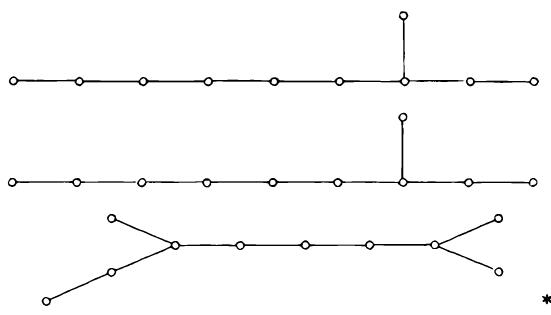
\includegraphics[keepaspectratio]{images/part001_3a8f46b0.jpg}}

¶ 18) Assume that (W,S) is of hyperbolic type, and that W leaves stable a lattice \(\Gamma\) of E. Let G be the orthogonal group of \(B_{M}\) , and let \(G(\Gamma)\) be the subgroup of elements \(g \in G\) such that \(g\Gamma = \Gamma\) . Show that \(G(\Gamma)\) is a discrete subgroup of G. Show that W is a subgroup of finite index of \(G(\Gamma)\) (use the fact that the measure of W\textbackslash G is finite).

*If (W, S) is actually of compact hyperbolic type, show that the corresponding Coxeter graph is isomorphic to one of the following (use Exercs. 4, 6 and 15):

\pandocbounded{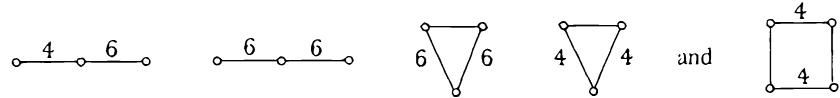
\includegraphics[keepaspectratio]{images/part001_0d92fd3d.jpg}}

Show that all the groups corresponding to the graphs of Exerc. 16 (with the exception of the last four) leave stable a lattice (use the method of Exerc. 6).*

\begin{enumerate}
\def\labelenumi{\arabic{enumi})}
\setcounter{enumi}{18}
\tightlist
\item
  Let \((W,S)\) be the Coxeter system corresponding to the graph
\end{enumerate}

\pandocbounded{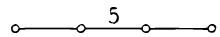
\includegraphics[keepaspectratio]{images/part001_8b3dcc37.jpg}}

This is a system of compact hyperbolic type (cf.~Exerc. 15). The coefficients of the form \(B_{M}\) with respect to the basis \((e_{s})\) belong to the subring A of the field \(\mathbf{Q}(\sqrt{5})\) consisting of the elements of this field that are integers over Z.

\begin{enumerate}
\def\labelenumi{\alph{enumi})}
\item
  Let \(\sigma\) be the embedding of \(K\) into \(\mathbf{R}\) that maps \(\sqrt{5}\) to \(-\sqrt{5}\) . Show that the transform \(\sigma(B_M)\) of the form \(B_M\) by \(\sigma\) is non-degenerate and positive.
\item
  Let G be the orthogonal group of \(B_{M}\) , and let \(G_{\sigma}\) be that of \(\sigma(B_{M})\) . Let \(G_{A}\) be the subgroup of G consisting of the elements whose matrices with respect to \((e_{s})\) have coefficients in A. Show that \(G_{A}\) can be identified with a discrete subgroup of \(G \times G_{\sigma}\) and then, using a), show that \(G_{A}\) is a discrete subgroup of G.
\item
  Show that W is a subgroup of \(G_{A}\) of finite index.
\end{enumerate}

\(d)\) Prove analogous results for the other graphs in Exerc. 15 (the field \(\mathbf{Q}(\sqrt{5})\) sometimes being replaced by \(\mathbf{Q}(\sqrt{2})\) , with the exception of the graph

\pandocbounded{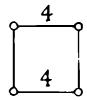
\includegraphics[keepaspectratio]{images/part001_99b486d1.jpg}}

treated in Exerc. 18, and of the graph \(^{8}\)

\pandocbounded{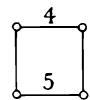
\includegraphics[keepaspectratio]{images/part001_2a5e784a.jpg}}

¶ 20) For every subset \(\{s, s'\}\) of S such that \(m(s, s') = \infty\) , let \(r(s, s')\) be a real number \(\leqslant -1\) . Equip E with the bilinear form \(\mathbf{B}_r\) such that

\[
\begin{array}{l l} \mathrm{B} _ {r} (e _ {s}, e _ {s ^ {\prime}}) = \mathrm{B} _ {\mathrm{M}} (e _ {s}, e _ {s ^ {\prime}}) = - \cos \frac {\pi}{m (s , s ^ {\prime})} & \text {if} m (s, s ^ {\prime}) \neq \infty \\ \mathrm{B} _ {r} (e _ {s}, e _ {s ^ {\prime}}) = r (s, s ^ {\prime}) & \text {if} m (s, s ^ {\prime}) = \infty . \end{array}
\]

We define, as for \(B_{M}\) , the reflections \(\sigma_{s}\) with vector \(e_{s}\) , leaving the form \(B_{r}\) invariant.

\begin{enumerate}
\def\labelenumi{\alph{enumi})}
\item
  Show that there exists a unique homomorphism \(\sigma_r: \mathbf{W} \to \mathbf{GL}(\mathbf{E})\) such that \(\sigma_r(g_s)\) is equal to the reflection \(\sigma_s\) defined above.
\item
  Show that the assertions in Prop. 4, Th. 1, its Corollaries, and Lemma 1 remain true for \(\sigma_r\) .
\end{enumerate}

